\documentclass[11pt]{article}

% some definitions for the title page
\newcommand{\reporttitle}{NLP Models}
\newcommand{\reportdescription}{Including LSTMs amd GRUs}

% load some definitions and default packages
%---------------------------------------------------------------------------
%	PACKAGES AND OTHER DOCUMENT CONFIGURATIONS
%---------------------------------------------------------------------------

\usepackage[twoside]{fancyhdr}
\usepackage{csquotes}

\usepackage[a4paper,hmargin=2.0cm,vmargin=1.0cm,includeheadfoot]{geometry}
% \usepackage{natbib} % for bibliography
\usepackage{biblatex}
\usepackage{tabularx,longtable,multirow,subfigure,caption}%hangcaption
\usepackage{fancyhdr} % page layout
\usepackage{url} % URLs
\usepackage[english]{babel}
\usepackage{graphicx}
\usepackage{rotating}
\usepackage{dsfont}
\usepackage{epstopdf} % automatically replace .eps with .pdf in graphics
% \usepackage{backref} % needed for citations
\usepackage{array}
\usepackage{latexsym}
\usepackage[pdftex,hypertexnames=false,colorlinks]{hyperref} % provide links in pdf (had pagebackref)
\usepackage{booktabs}
\usepackage{wrapfig}
\usepackage{caption}  % Required for \captionof
\usepackage{float} % for H option in figures
\usepackage{amssymb}
\usepackage{amsmath}
\usepackage{amsthm}
\usepackage{mathtools} % for 'dcases*' env.
\usepackage[nottoc]{tocbibind}

%%% Default fonts
\renewcommand*{\rmdefault}{bch}
\renewcommand*{\ttdefault}{cmtt}

%%% Default settings (page layout)
\setlength{\parindent}{0em}  % indentation of paragraph
\setlength{\parskip}{.3em}
\setlength{\itemsep}{0.mm}

\setlength{\headheight}{14.5pt}
\pagestyle{fancy}

\fancyfoot[ER,OL]{\thepage}%Page no. in the left on odd pages and on right on even pages

\fancyfoot[OC,EC]{\sffamily }
\renewcommand{\headrulewidth}{0.1pt}
\renewcommand{\footrulewidth}{0.1pt}
\captionsetup{margin=10pt,font=small,labelfont=bf}

% LISTINGS ammendments
\usepackage{listings}
\usepackage{color}

\definecolor{mygreen}{rgb}{0,0.6,0}
\definecolor{mygray}{rgb}{0.5,0.5,0.5}
\definecolor{mymauve}{rgb}{0.58,0,0.82}

\lstset{ 
  postbreak=\mbox{\textcolor{red}{$\hookrightarrow$}\space},
  backgroundcolor=\color{white},   % choose the background color; you must add \usepackage{color} or \usepackage{xcolor}; should come as last argument
  basicstyle=\footnotesize,        % the size of the fonts that are used for the code
  breakatwhitespace=false,         % sets if automatic breaks should only happen at whitespace
  breaklines=true,                 % sets automatic line breaking
  captionpos=b,                    % sets the caption-position to bottom
  commentstyle=\color{mygreen},    % comment style
%   deletekeywords={...},            % if you want to delete keywords from the given language
%   escapeinside={\%*}{*)},          % if you want to add LaTeX within your code
  extendedchars=true,              % lets you use non-ASCII characters; for 8-bits encodings only, does not work with UTF-8
  firstnumber=1,                % start line enumeration with line 1000
  frame=single,	                   % adds a frame around the code
  keepspaces=true,                 % keeps spaces in text, useful for keeping indentation of code (possibly needs columns=flexible)
  columns=fullflexible,
  keywordstyle=\color{blue},       % keyword style
  language=python,                 % the language of the code
  % morekeywords={*,...},            % if you want to add more keywords to the set
  numbers=left,                    % where to put the line-numbers; possible values are (none, left, right)
  numbersep=5pt,                   % how far the line-numbers are from the code
  numberstyle=\tiny\color{mygray}, % the style that is used for the line-numbers
  rulecolor=\color{black},         % if not set, the frame-color may be changed on line-breaks within not-black text (e.g. comments (green here))
  showspaces=false,                % show spaces everywhere adding particular underscores; it overrides 'showstringspaces'
  showstringspaces=false,          % underline spaces within strings only
  showtabs=false,                  % show tabs within strings adding particular underscores
  stepnumber=1,                    % the step between two line-numbers. If it's 1, each line will be numbered
  stringstyle=\color{mymauve},     % string literal style
  tabsize=2,	                   % sets default tabsize to 2 spaces
  title=\lstname% show the filename of files included with \lstinputlisting; also try caption instead of title
}

% Here, you can define your own macros. Some examples are given below.

\newcommand{\R}[0]{\mathds{R}} % real numbers
\newcommand{\Z}[0]{\mathds{Z}} % integers
\newcommand{\N}[0]{\mathds{N}} % natural numbers
\newcommand{\C}[0]{\mathds{C}} % complex numbers
\renewcommand{\vec}[1]{{\boldsymbol{{#1}}}} % vector
\newcommand{\mat}[1]{{\boldsymbol{{#1}}}} % matrix


\bibliography{../bibliography}

\begin{document}

% Include the title page
\begin{titlepage}

    \newcommand{\HRule}{\rule{\linewidth}{0.5mm}} % Defines a new command for the horizontal lines, change thickness here
    
    \center % Center everything on the page
     
    %------------------------------------------------------------------------
    %	HEADING SECTIONS
    %------------------------------------------------------------------------
    
    \textsc{\Large Department of Computing}\\[0.5cm] 
    \textsc{\large Imperial College of Science, Technology and Medicine}\\[0.5cm] 
    
    %------------------------------------------------------------------------
    %	TITLE SECTION
    %------------------------------------------------------------------------
    
    \HRule \\[0.4cm]
    { \huge \bfseries \reporttitle}\\ % Title of your document
    \HRule \\[0.4cm]

    \textit{\reportdescription}
    
    \vspace{2em}

    %------------------------------------------------------------------------
    %	AUTHOR SECTION
    %------------------------------------------------------------------------
    
    \large \emph{Author: Anton Zhitomirskiy}

    \vspace{1em}

    \global\let\newpagegood\newpage
    \global\let\newpage\relax
    
\end{titlepage}

\global\let\newpage\newpagegood

\tableofcontents

\clearpage

\section{Sparsity}

\subsection{Problem}

WSJ corpus: built over 10 years ago. What would happen if tested on today’s News articles?

If certain words are absent then the proability in the n-gram is zero. We can use smoothing to solve this or give it unknown word tokens. 
% Alternatively, we can give an unknown word token (but these have to be in the training set and the test set). This unknown word is used if a word appears to little times, or we apply this directly to our vocabulary set.

\subsection{Add-one smoothing}

\begin{figure}[H]
    \centering
    \subfigure[Counts after one-smoothing (we've added +1 to EVERYTHING)]{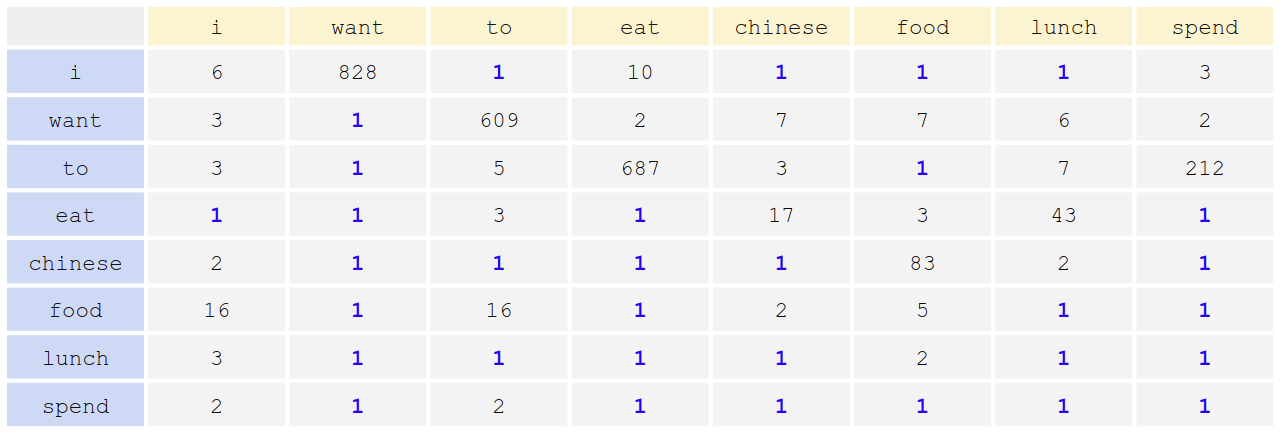
\includegraphics[width=.8\linewidth]{figures/after-one-smoothing.png}}
    \subfigure[probabilities before one-smoothing]{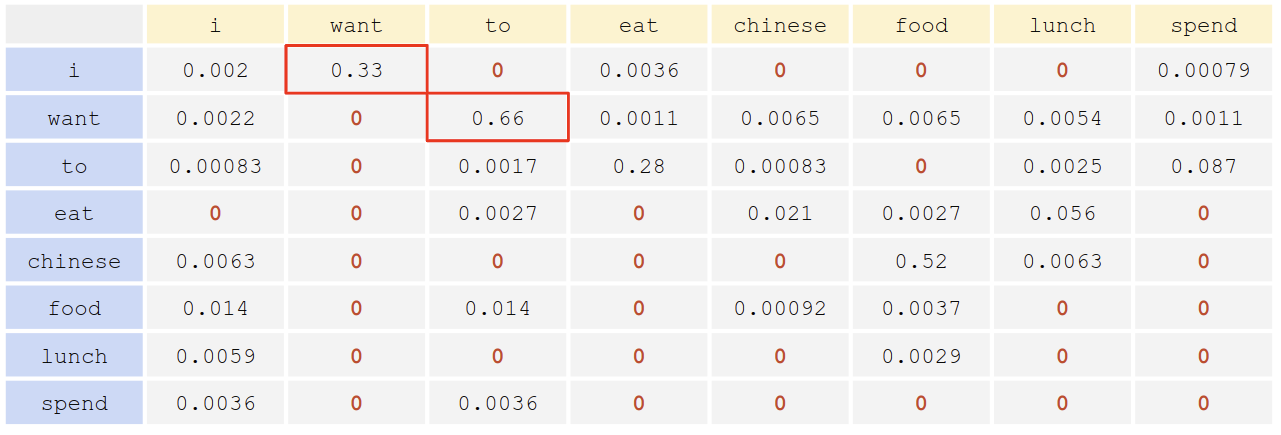
\includegraphics[width=.8\linewidth]{figures/before-one-smoothing.png}}
    \subfigure[probabilities after one-smoothing]{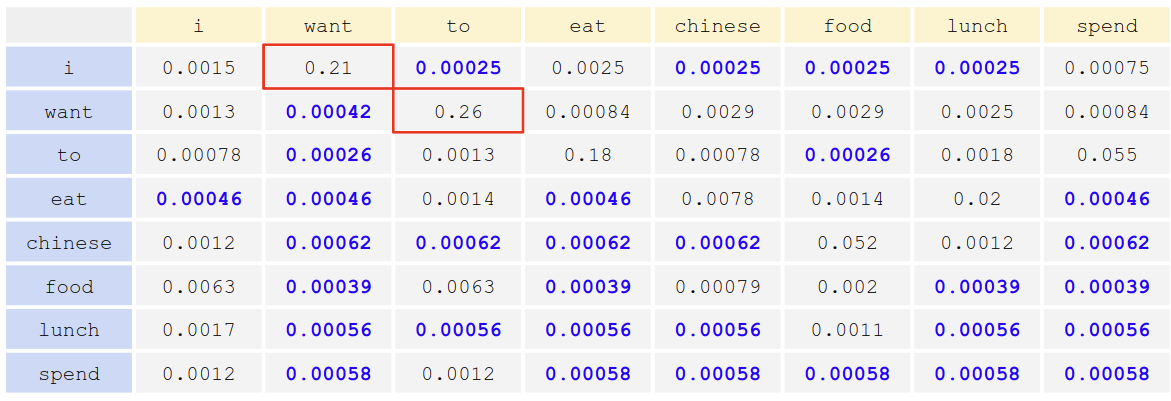
\includegraphics[width=.8\linewidth]{figures/after-one-smoothing-probs.png}}
    \subfigure[total instances of words]{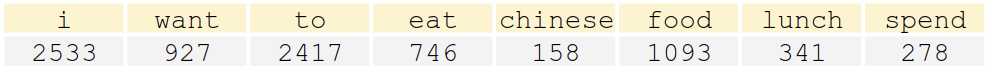
\includegraphics[width=.8\linewidth]{figures/bi-gram-total.png}}
    \caption{difference between smoothing and not}\label{fig:smoothing-example}
\end{figure}

\begin{equation*}
    P_{add-1}(w_n|w_{n-1})=\frac{C(w_{n-1},w_n)+1}{C(w_{n-1})+V}
\end{equation*}

Given words with sparse statistics, they steal probability mass from more frequent words. This is because smaller instances of vocabulary are more influenced by the V and +1 term appearing in the new fraction. However, for larger occurrences they shrink because the nominator is large (so +1) won't change it by much, but the denominator grows larger, making the overall probability less.

The change here is great between the hilighted terms in Figure~\ref{fig:smoothing-example}. ``If we have very few instances of the word `want' the smoothing will impact this a lot and this number will therefore change a lot. Wheras, if we have a lot of counts within the word `i' then it wont change the probability a lot.'' Indeed, looking at the total instances of word i, the denominator is so large already that the number wasn't impacted, and `want' was impacted.

\subsubsection{Problems}

Although easy to implement, it takes too much probability mass from more likely occurrences (see Figure~\ref{fig:smoothing-example}) and assigns too much probability to unseen events. Therefore, we could try +k smoothing witha  smaller value of k.

\subsection{Back-off smoothing}

If we don't have any occurrences in our current (trigram) model, we can back-off and see how many occurrences there are in the smaller (bigram) model.

\begin{definition}[Back off smoothing ``sutpid back-off'']
    \begin{align*}
        S(w_i|w_{i-2}w_{i-1}) &=
        \begin{cases}
            \frac{C(w_{i-2}w_{i-1}w_i)}{C(w_{i-2}w_{i-1})} , & if\ C(w_{i-2}w_{i-1}w_i) > 0 \\
            0.4 \cdot S(w_i|w_{i-1}) , & otherwise    
        \end{cases} \\
        S(w_i|w_{i-1}) &=
        \begin{cases}
            \frac{C(w_{i-1}w_i)}{C(w_{i-1})} , & if\ C(w_{i-1}w_i) > 0 \\
            0.4 \cdot S(w_i) , & otherwise    
        \end{cases} \\
        s(w_i) &= \frac{C(w_i)} N
    \end{align*}    

    \begin{warning}
        Note, this is not a probability, but a score
    \end{warning}
\end{definition}

Where $N$ is the number of words in the text

\subsubsection{Problems}

suppose that the bigram ``a b'' and the unigram ``c'' are very common, but the trigram ``a b c'' is never seen. Since ``a b'' and ``c'' are very common, it may be significant (that is, not due to chance) that ``a b c'' is never seen.

Perhaps it's not allowed by the rules of the grammar.  Instead of assigning a more appropriate value of 0, the method will back off to the bigram and estimate $P(c | b)$, which may be too high

\subsection{Interpolation}

Combine evidence from different n-grams:

\begin{definition}[Interpolation]
    \begin{equation*}
        P_{interp}(w_i|w_{i-2}w_{i-1})=\lambda_1 P(w_i|w_{i-2} w_{i-1}) + \lambda_2 P(w_i|w_{i-1}) + \lambda_3 P(w_i), \quad where\ \lambda_1 + \lambda_2 + \lambda_3 = 1
    \end{equation*}
\end{definition}

\section{Feed-forward neural language models}

\begin{figure}[H]
    \centering
    \subfigure[Lecture diagram]{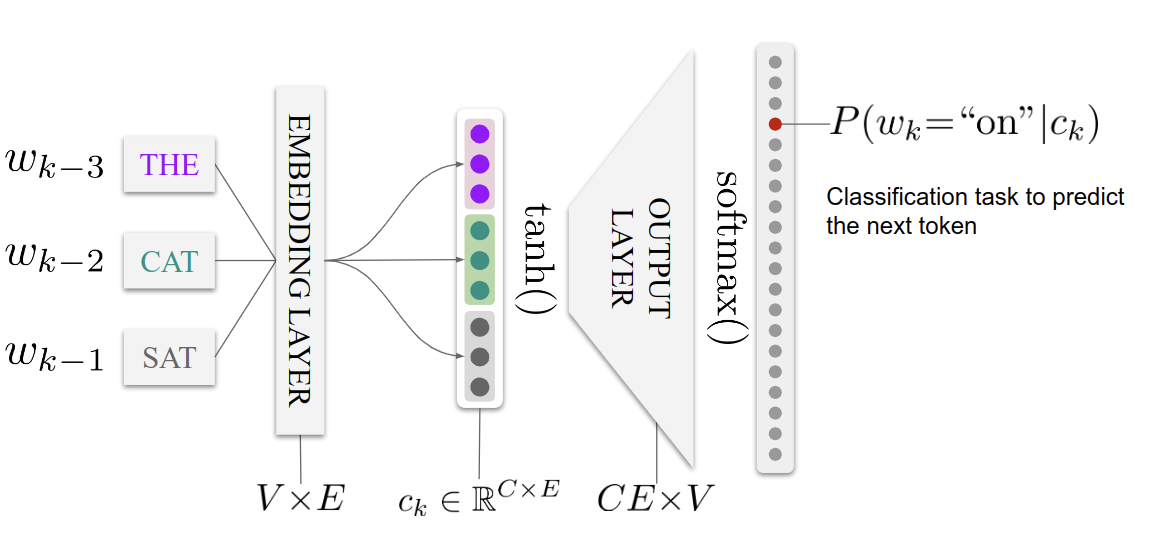
\includegraphics[width=.8\linewidth]{figures/FFLM-lecture.png}}
    \subfigure[Paper diagram~\cite{FFLM-2003}]{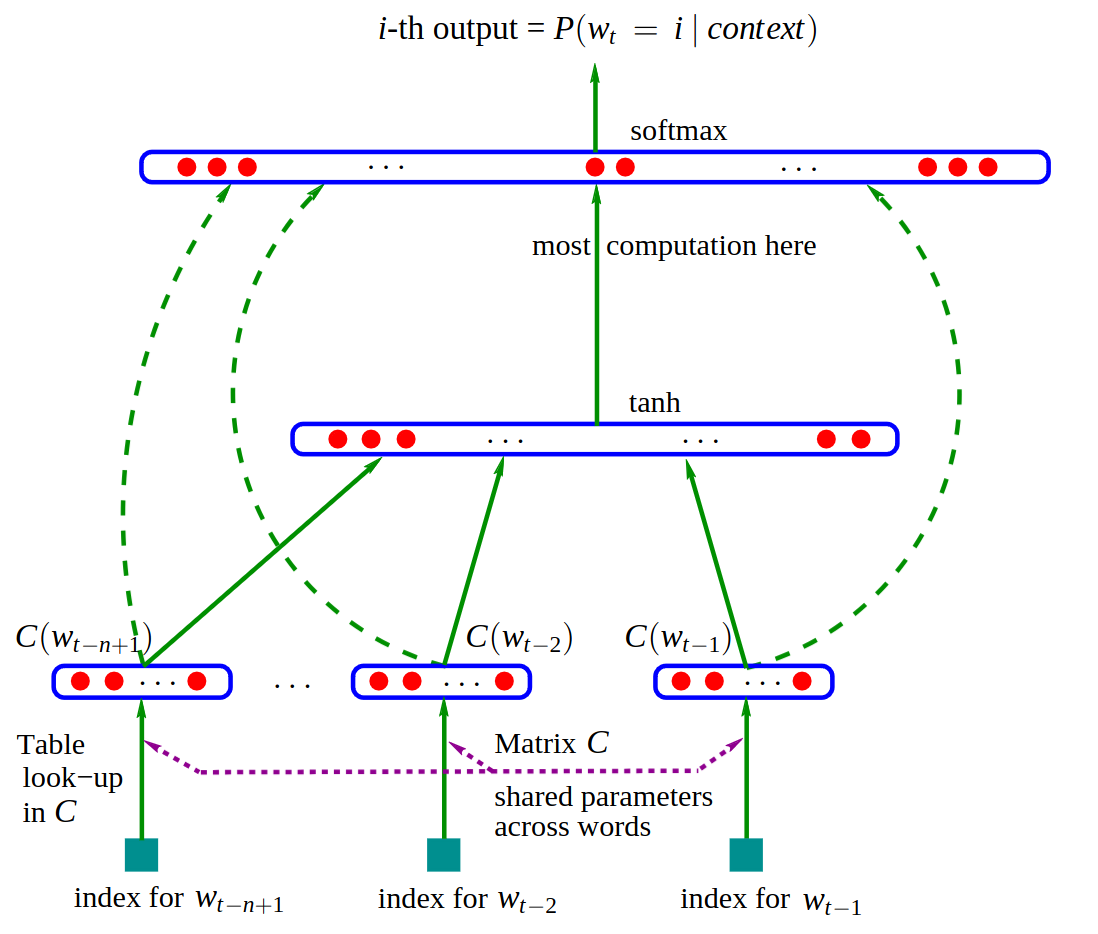
\includegraphics[width=.8\linewidth]{figures/FFLM-paper.png}}
    \caption{FFLM diagrams}\label{fig:fflm}
\end{figure}

It approximates history with last C words (C affects model size) e.g. 4-gram FFLM has a context size of 3. The context is formed by concatenating word embeddings.

\section{Vanilla RNNs for language modelling}

\begin{figure}[H]
    \centering
    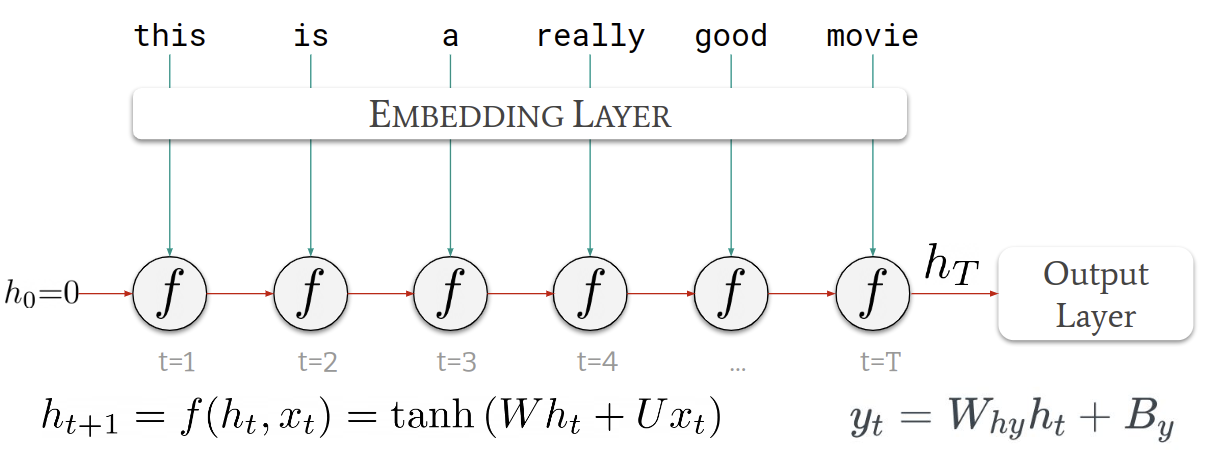
\includegraphics[width=\linewidth]{figures/Rnn-architecture.png}
\end{figure}

Before we had classifciation, each function took a hidden state and output this into the output layer. We could do this differently, but instead of taking the final we could max on each dimension also.

\subsection{Many-to-many RNN}

Every input has a label, in languag emodelling you predict the next word. The LM loss is predicted form the cross-entropy losses from each timestep.

\begin{figure}[H]
    \centering
    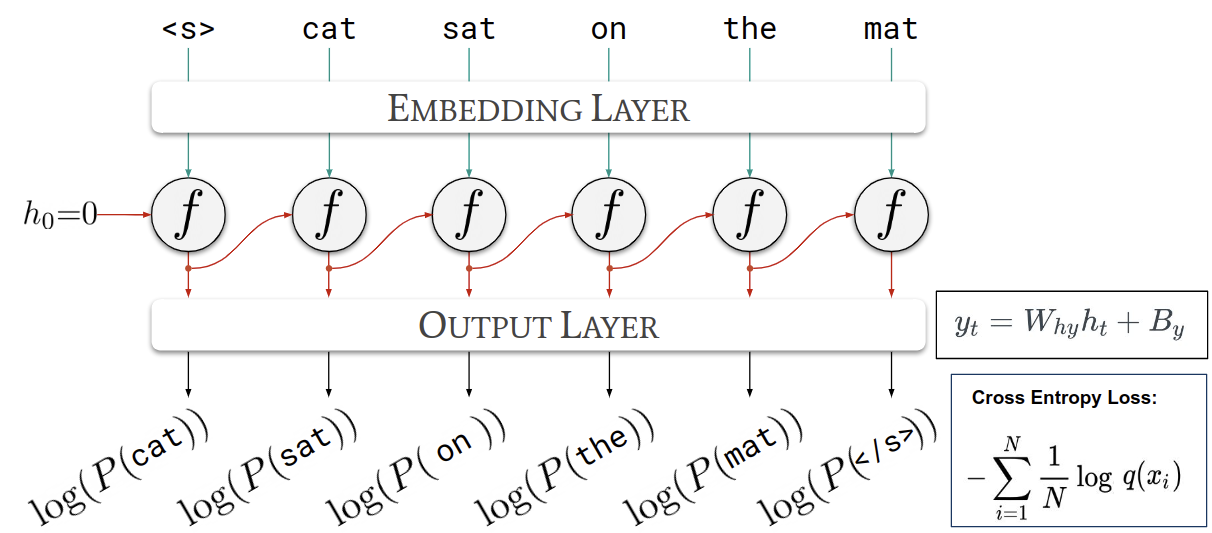
\includegraphics[width=\linewidth]{figures/rnn-mtm.png}
\end{figure}

In addition to passing the hidden state to the next funciton, you also use it in the output layer. The size of $W$: lets say the hidden state has H dimensions, it must go to the size of the vocab, becuase you're predicting which word is going to come next out of the whole vocab, so it is $V\times H$.

We take the log probabilities because you want to use the cross entropy loss (which is the average across the outputs)

\subsubsection{Teacher forcing}

In the event where this network predicts an incorrect label some way along the prediction, we force it to use the actual expected label because otherwise the network would be learning some strange behaviour if you are given incorrect predictions somewhere along the line.

If you don't use it, then there is instability in the model.

\subsubsection{Weight tying, reducing the no. of parameters}

We have very big models; big vocabulary causes matricies of dimension $V\times \cdot$.

We can use the same embedding weights in our output layer: ($E$ has dimensions: $H \times |V|$). If you have a matrix $E$ that maps from a one-hot vector into an embedding, you can use E transpose in the output layer.

\begin{align*}
    & e_t & = & Ex_t & \\ 
    & h_{t+1} & = & \tanh(Wh_t + Ue_t) & \\
    & y_t & = & softmax(E^\top h_t) & E^\top \text{ has dimensions}: |V| \times H
\end{align*}

U could be from the size of the imbedding to the size of the hidden state, but if we do the weight tying then it has to be $H \times H$.

\section{Bi-directional RNNs}

\subsection{Bi-directional RNNs}

\begin{figure}[H]
    \centering
    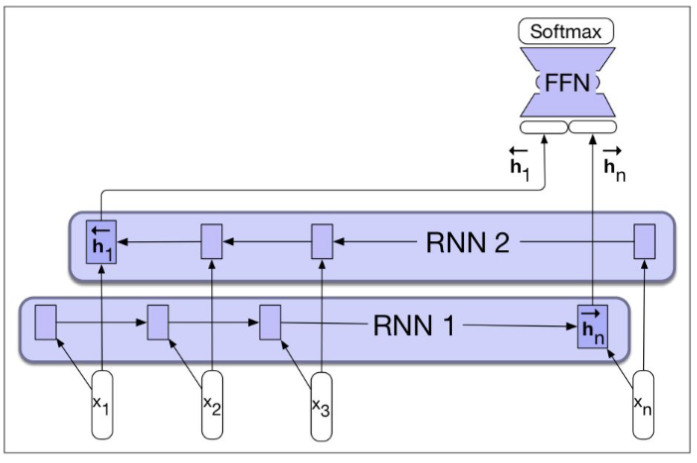
\includegraphics[width=\linewidth]{figures/bi-directional-rnn.png}
\end{figure}

We can concatenate the representations at the end of the RNNs for both directions. 

When comparing the number of parameters in this vs a single directional rnn, it doubles. The output layer also doubles (because we are given a matrix $H\times O$ twice from each direction making the output layer have dimension $H\times H \times O$).

\subsection{Multi-layered RNNs}

\begin{figure}[H]
    \centering
    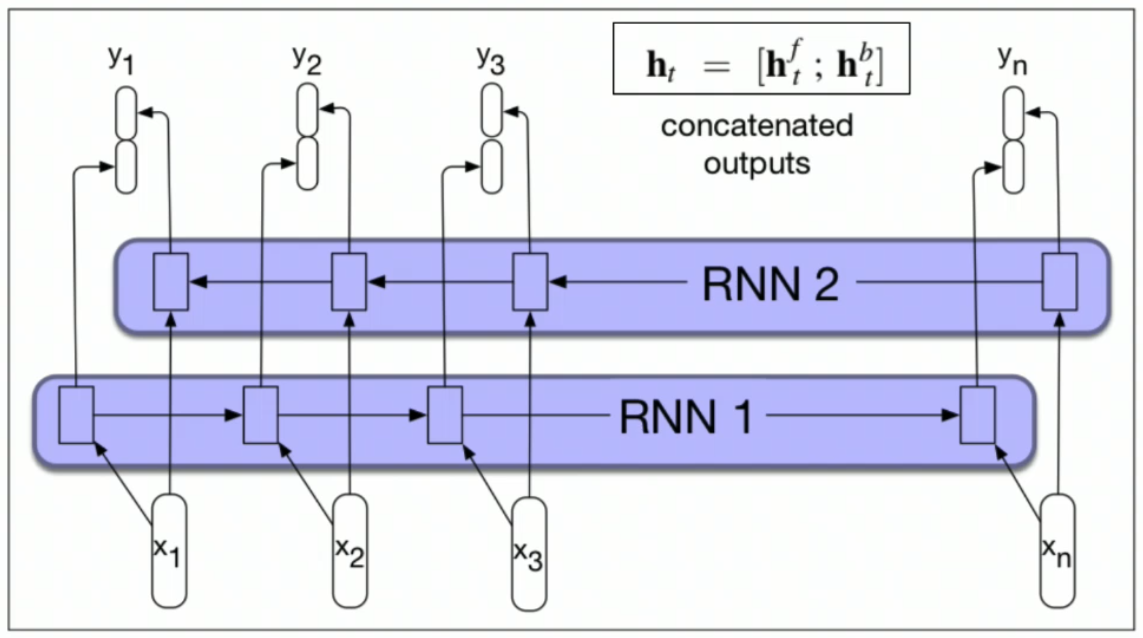
\includegraphics[width=\linewidth]{figures/rnn-bidirectional-not-single-output.png}
\end{figure}

We can also predict every single token (every word we input). We concattenate them and can make a prediction at each time step. Then, following this, we can stack networks on-top of eachother.

\begin{figure}[H]
    \centering
    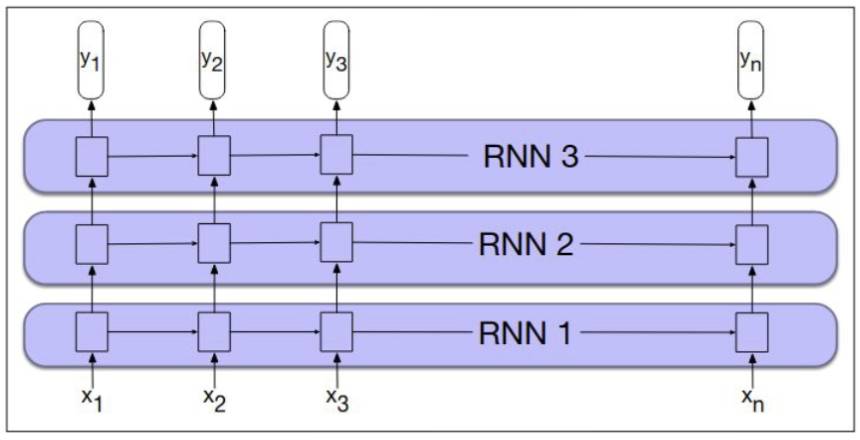
\includegraphics[width=\linewidth]{figures/multi-layered-rnn.png}
\end{figure}

\subsection{Bi-directional multi-layered RNNs}

\begin{figure}[H]
    \centering
    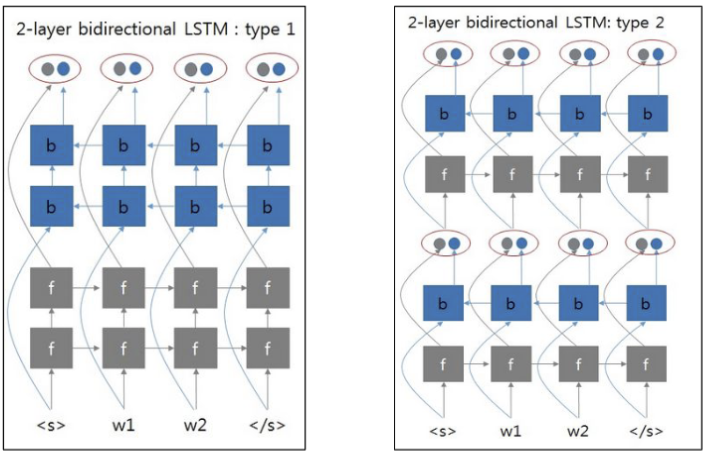
\includegraphics[width=\linewidth]{figures/bi-directional-multi-layered-rnn.png}
\end{figure}

Currently forward output and backward output is concatenated after each layer. But, for language modeling, we need independent forward rnn and backward rnn util the last layer and output concatenation is only need at the last layer.

\section{LSTMs}

\begin{figure}[H]
    \centering
    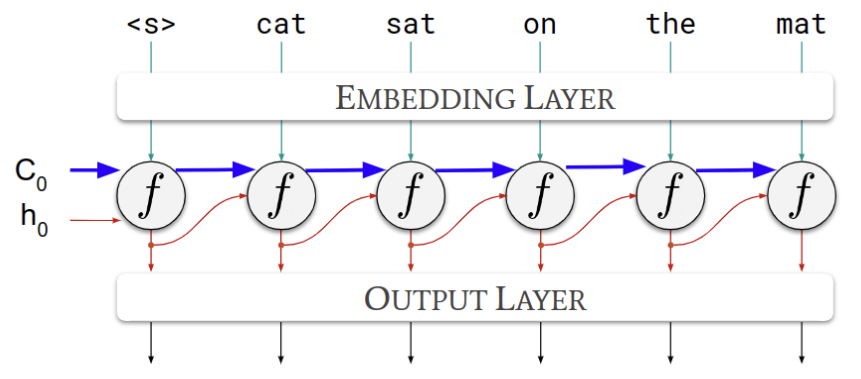
\includegraphics[width=\linewidth]{figures/lstm.png}
\end{figure}

Cell states ($C_t$) represnt `long term memory', and hidden states ($h_t$) is current working memory (same as for vanilla RNN).

\subsection{How it works}

\subsubsection{Step 1: we start from what we know already}

We used vanilla rnns before. The current value is:

\begin{equation*}
    g_t = \tanh(W_{ig}x_t + W_{hg}h_{t-1} + b_g)
\end{equation*}

\subsubsection{Step 2: we define our cell state}

With LSTM, we also want a cell state for long term memory

\begin{equation*}
    c_t = f_t \ast c_{t-1} + i_t \ast g_t
\end{equation*}

We define this by the cell state from the previous time step $c_{t-1}$ and add it to some of what we got form this time step $g_t$ with some multiplier for each of those.

The model can now choose to keep this state the same or forget everything. 

Note that $f_t \wedge i_t$  are in terms of t so they're not the same every time step - so we can choose when to remember or when to forget. The decision should be based on what the input is for that time step and what the context is up to thtat point.

\subsubsection{Step 2. The forget gate}

$f_t$ is the forget gate, and is a vector between 0 and 1. It needs to consider $x_t \wedge h_{t-1}$ and returns a vector between 0 and 1.

\begin{equation*}
    f_t = \sigma (W_{if}x_t + W_{hf}h_{t-1}+b_f)
\end{equation*}

\subsubsection{Step 2. The input gate}

Similarly, with $i_t$ it is the input gate and is a vector between 0 and 1.

\begin{equation*}
    fi_t = \sigma (W_{ii}x_t + W_{hi}h_{t-1}+b_i)
\end{equation*}

\subsubsection{Step 3. prepare next hidden state}

Here, we are transforming $c_t$ to give us $h_t$. 

\begin{equation*}
    h_t = o_t \ast \tanh(c_t) 
\end{equation*}

\subsection{Full equations}

\begin{align*}
    i_t & = \sigma (W_{ii}x_t + W_{hi}h_{t-1}+b_i) \\
    f_t & = \sigma (W_{if}x_t + W_{hf}h_{t-1}+b_f) \\
    o_t & = \sigma (W_{io}x_t + W_{ho}h_{t-1}+b_o) \\
    g_t & = \tanh(W_{ig}x_t + W_{hg}h_{t-1}+b_g)
\end{align*}

\begin{align*}
    c_t & = f_t \ast c_{(t-1)} + i_t \ast g_t \\
    h_t & = o_t \ast \tanh(c_t)
\end{align*}

\subsubsection{Dimensions}

If we have $E$ dimensional embeddings and $H$ dimensional vectors.

\begin{itemize}
    \item $W_{ii}=(H\times E)$ is the weight matrix applied to the input. We go from the embeddings to $i_t$. We know that $i_t$ is $H$ dimensional 
    \item $W_{hi}=(H\times H)$ is the weight matrix applied to the input gate whose dimensions must match the addition of the step prior, 
\end{itemize}

\textbf{EXAMPLE}

If we have 100 dimensional hidden states, 500 dimensional embeddings and a classificaiton taks with 5 classes (no bias term in the output layer), then excluding any embedding layer, how many parameters do we have?

Look at the dimensions of the weight matricies, we have $100 \times 500$ and $100 \times 100$. The bias term in these intermediate hidden layers is therefore 100 also. Then similarly for the rest so $(100 \times 500 + 100 \times 100 + 100)\times 4$.

In the output layer, we have 5 output classes, so we must convert from having $H$ dimensions to $5$ dimensions in our weight matrix i.e. $100\times 5$.

Therefore, we have $24,900$ parameters.

\textbf{EXAMPLE BIDIRECTIONAL}

Same as above, only we multiply by 2 in the hidden layers, and 2 once again in the output layer because we're getting data sent in from two streams, each without output dimension $H$.

\subsection{Why do LSTMs help with vanishing gradients?}

The gradients thorugh the cell states are hard to vanishing
\begin{enumerate}
    \item Additive formula means we don't ahve repeated multiplication of the same matrix (we have a derivative thats more `well behaved')
    \item The forget gate means that our model can learn when to let the gradients vanish, and when to preseve them .This gate can take different values at different time steps.
\end{enumerate}

\section{GRU}

\subsection{How it works}

Similar, only instead of having two distinct gates, we have $z_t \wedge (1-z_t)$. Also we have a update gate $r_t$.

\subsubsection{Step 1. Current value}

\begin{equation*}
    g_t = \tanh(W_{ig}x_t + r_t \ast (W_{hg}h_{t-1} + b_g))
\end{equation*}

\subsubsection{Step 1. Update gate}

How much do we consdier the previous hidden state

\begin{equation*}
    r_t = \sigma(W_{ir}x_t + W_{hr}h_{t-1} + b_r)
\end{equation*}

\subsubsection{Step 2. Long term memory}

Our long term memory is only controlled by a reset gate ($z_t$)

\begin{equation*}
    h_t = (1-z_t) \ast g_t + z_t \ast h_{t-1}
\end{equation*}

\subsubsection{Step 2. Reset gate}

\begin{equation*}
    z_t = \sigma(W_{iz}x_t + W_{hz}h_{t-1} + b_z)
\end{equation*}

\subsubsection{No output gate}


\section{Revision \& little tangent on de-biasing}

\printbibliography
\addcontentsline{toc}{section}{Bibliography}

\end{document}